\chapter{Estado del arte}

El estado del arte se basa en el estudio de la técnica de \emph{video mapping} y del modelado automático de geometrías.
El proceso de creación de un espectáculo de \emph{video mapping} se apoya en entrevistas a \emph{VJs} y en un relevamiento de las aplicaciones por ellos sugeridas, anexadas en los apéndices \titleref{chapter:aportes} y \titleref{chapter:aplicaciones} respectivamente.
Por su parte, el modelado automático es un área no solo relacionada al \emph{video mapping} sino que es aplicable también en distintas ramas de la ingeniería como son la visión por computadora, animación tridimensional, interfaces persona-computadora, entre otras. Es por esta razón que se decidió realizar un estudio de estas técnicas, abordándose de forma genérica los problemas de obtención de una nube de puntos$^\dagger$ correspondientes a objetos tridimensionales reales y la reconstrucción de mallas$^\dagger$ tridimensionales para su utilización durante el proceso de creación de espectáculos.

\section{Creación de un espectáculo de \emph{video mapping}}

La creación de un espectáculo de \emph{video mapping} se presenta en tres etapas: el modelado de la escena, la producción del espectáculo y la proyección del mismo.
Cada una de estas etapas será abordada en esta sección desde dos enfoques: bidimensional y tridimensional, ya que tanto los problemas que plantean, así como los escenarios de aplicación difieren en cada caso, según el enfoque.

Durante la etapa de modelado de la escena, se obtiene una representación abstracta de los objetos reales sobre los que se proyectará. Este modelo constituye la base para trabajar en posteriores etapas y sobre él se diseñará el espectáculo.

La producción del espectáculo consiste en definir los distintos efectos visuales a ser aplicados sobre los objetos modelados y la forma en que serán ejecutados. Los espectáculos pueden discriminarse en dos categorías según la forma de presentación de los efectos pudiendo ser en una secuencia predefinida o en tiempo real.
Si la secuencia a ejecutar es predefinida, en esta etapa se define dicha secuencia indicando el instante en que cada efecto se desplegará. Esto por lo general se hace de forma sincronizada con la música que suele acompañar al espectáculo. Por otra parte, si la ejecución de los efectos se define en tiempo real, esta etapa es utilizada para definir los mecanismos que desencadenan la ejecución de los efectos. Así por ejemplo, se podría definir para un teclado, un efecto distinto para cada tecla para que el \emph{VJ} los ejecute a voluntad en la presentación.
En esta etapa también se diseña y produce la musicalización que será utilizada durante todo el espectáculo.

Es en la etapa de proyección del espectáculo en donde se puede contemplar el resultado de los distintos efectos visuales proyectados sobre las superficies, acompañados estos por efectos de sonido. Para lograr la correspondencia en la proyección de los objetos del modelo con las superficies se debe calibrar la proyección.
Esto se logra modificando el modelo de la escena, ajustando la posición y orientación de los proyectores, así como los parámetros intrínsecos de la proyección, siendo estos el ángulo de enfoque, la resolución y distancia focal.

\begin{figure}[H]
  \centering
    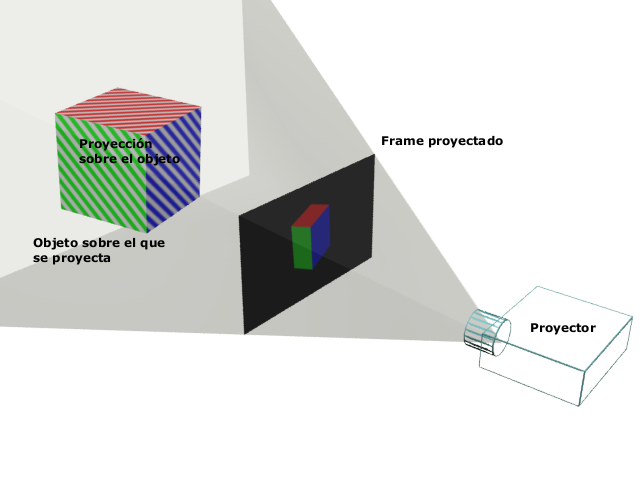
\includegraphics[width=0.7\textwidth]{./Cap2_videomapping/proy2dvs3d}
  \caption[Imagen propia]{Esquema de proyección.}
  \label{fig:proy2dvs3d}
\end{figure}

\subsection{Enfoque bidimensional}
\subsubsection{Modelo}
Un modelo bidimensional refleja lo que vería un observador desde un punto de vista fijo.
Técnicamente es el resultado de una proyección en perspectiva \cite{LibroCompGrafica} sobre un plano de vista de los elementos de la superficie a modelar.
Este punto de vista debe ser considerado al posicionar y orientar el proyector que reproducirá el espectáculo.
La posición, orientación y campo de vista del proyector definirán además la sección de superficie sobre la que se proyectará.
En caso de utilizar más de un proyector cada uno de estos será posicionado en un lugar diferente y por lo tanto será necesario un modelo por cada uno de ellos.

\begin{figure}[H]
  \centering
    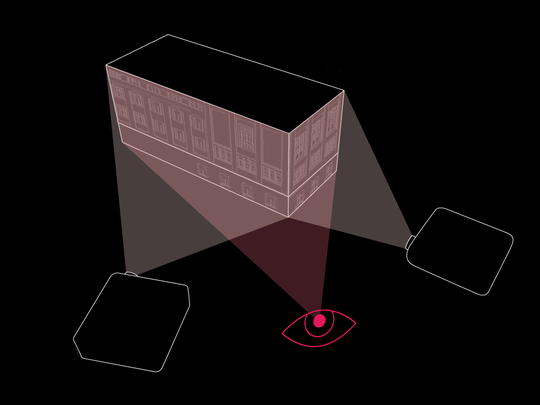
\includegraphics[width=0.7\textwidth]{./Cap2_videomapping/diagrama-2proyectores}
  \caption[vvvv.org]{Proyectores y sus puntos de vista.}
  \label{fig:diagrama-2proyectores}
\end{figure}

Son ejemplos de modelos: Fotografías, planos arquitectónicos y figuras geométricas.
Cada uno de estos requiere distintas técnicas para su creación y la forma de trabajo en las posteriores etapas dependerá del modelo utilizado.

Una fotografía captura lo que vería un observador desde el punto de vista desde donde fue tomada. Es una forma sencilla de crear el modelo de una escena, aunque usualmente requieren trabajo adicional para llegar a ser un modelo fiel. Para utilizar este modelo en etapas posteriores es conveniente que el punto de vista desde donde fue tomada la fotografía coincida con la posición desde donde se desea proyectar, de esta forma minimizando los ajustes de calibración necesarios.

Un plano arquitectónico, por ejemplo de una fachada, contiene información exacta de las medidas de la superficie que representa en una escala dada. Generalmente utiliza el método de proyecciones paralelas \cite{LibroCompGrafica} sobre un plano de proyección. Para utilizar el plano arquitectónico como modelo se debe transformar de forma que coincida con la proyección en perspectiva desde el punto vista donde estará ubicado el proyector.

Mediante figuras geométricas se modelan sectores de la superficie a proyectar. Un método para generarlas consiste en utilizar un proyector y herramientas de software que permiten delinear el contorno de las secciones de la superficie, ajustando el modelo en el momento de la construcción. Al usar el proyector para obtener el modelo queda incorporada la perspectiva del mismo por lo tanto no es necesaria otra calibración a menos de modificaciones en la ubicación u orientación del proyector.
Otro método consiste en dibujar las figuras con una fotografía o plano de fondo. En este caso la construcción de las figuras geométricas se realiza delineando el contorno de la superficie en la fotografía o plano.
Este tipo de modelos también pueden ser generados de forma automática utilizando técnicas de visión por computadora$^\dagger$ como por ejemplo el método basado en el filtrado de partículas\cite{ArticuloAutom2dmodel} para el reconocimiento de aristas.

\begin{figure}[H]
  \centering
	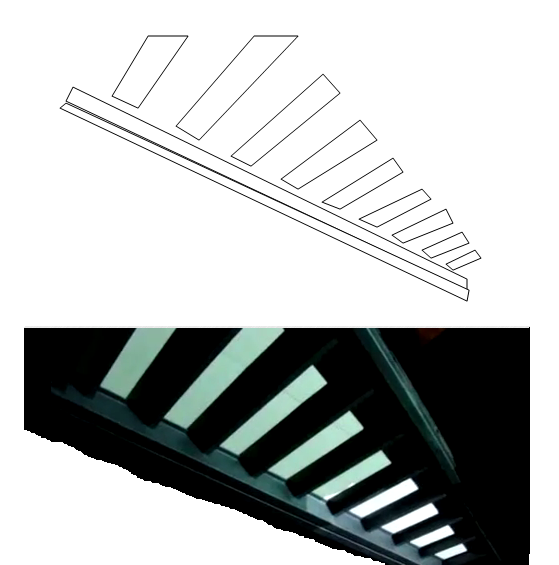
\includegraphics[width=0.7\textwidth]{./Cap2_videomapping/RepresentacionconfigurasGeometricas}
  \caption[Imagen propia]{Representación con figuras geométricas.}
  \label{fig:RepresentacionconfigurasGeometricas}
\end{figure}

\subsubsection{Producción del espectáculo}
La producción del espectáculo en dos dimensiones consiste en definir efectos visuales sobre regiones de un espacio bidimensional discreto$^\dagger$ representadas en el modelo de la escena. Este espacio se representa con coordenadas de pantalla que identifican cada uno de los píxeles$^\dagger$ del área de trabajo. Los efectos visuales se logran realizando cualquier animación computacional que genere una salida gráfica como pueden ser videos e imágenes.
En esta etapa, además de definir los efectos, se planifica cuando se mostrarán cada uno de ellos, pudiendo sincronizarse con la música que forma parte del espectáculo.
Los efectos podrán ser mostrados de forma secuencial, planificando en qué instante se ejecutará cada uno de ellos, o también definiendo acciones para que un \emph{VJ} decida en tiempo real en un espectáculo en vivo, los efectos a desplegar.

En computación gráfica se utilizan texturas para proyectar videos e imágenes sobre regiones del área de trabajo. Las texturas son mapas de bits$^\dagger$ utilizados para cubrir la superficie de un objeto virtual. Estos mapas de bits pueden ser generados a partir de imágenes, videos, o incluso dinámicamente mediante rutinas computacionales permitiendo así crear efectos visuales como, por ejemplo, la transición de un color a otro.

\begin{minipage}{0.50\textwidth}
	\begin{flushleft} \large
		\begin{figure}[H]
		  \centering
			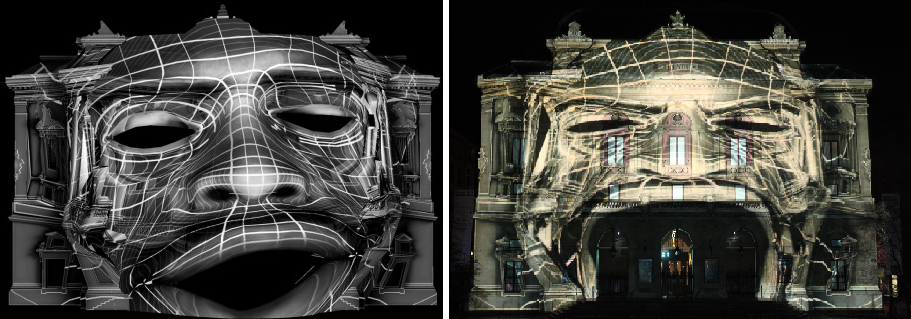
\includegraphics[width=0.7\textwidth]{./Cap2_videomapping/celestin_head.jpg}
		  \caption[http://mappingvideo.blogspot.com/]{Izq. Efecto en una herramienta de software. Der. Efecto proyectado.}
		  \label{fig:Efecto1}
		\end{figure}
	\end{flushleft}
\end{minipage}
\begin{minipage}{0.50\textwidth}
	\begin{flushright} \large
		\begin{figure}[H]
		  \centering
			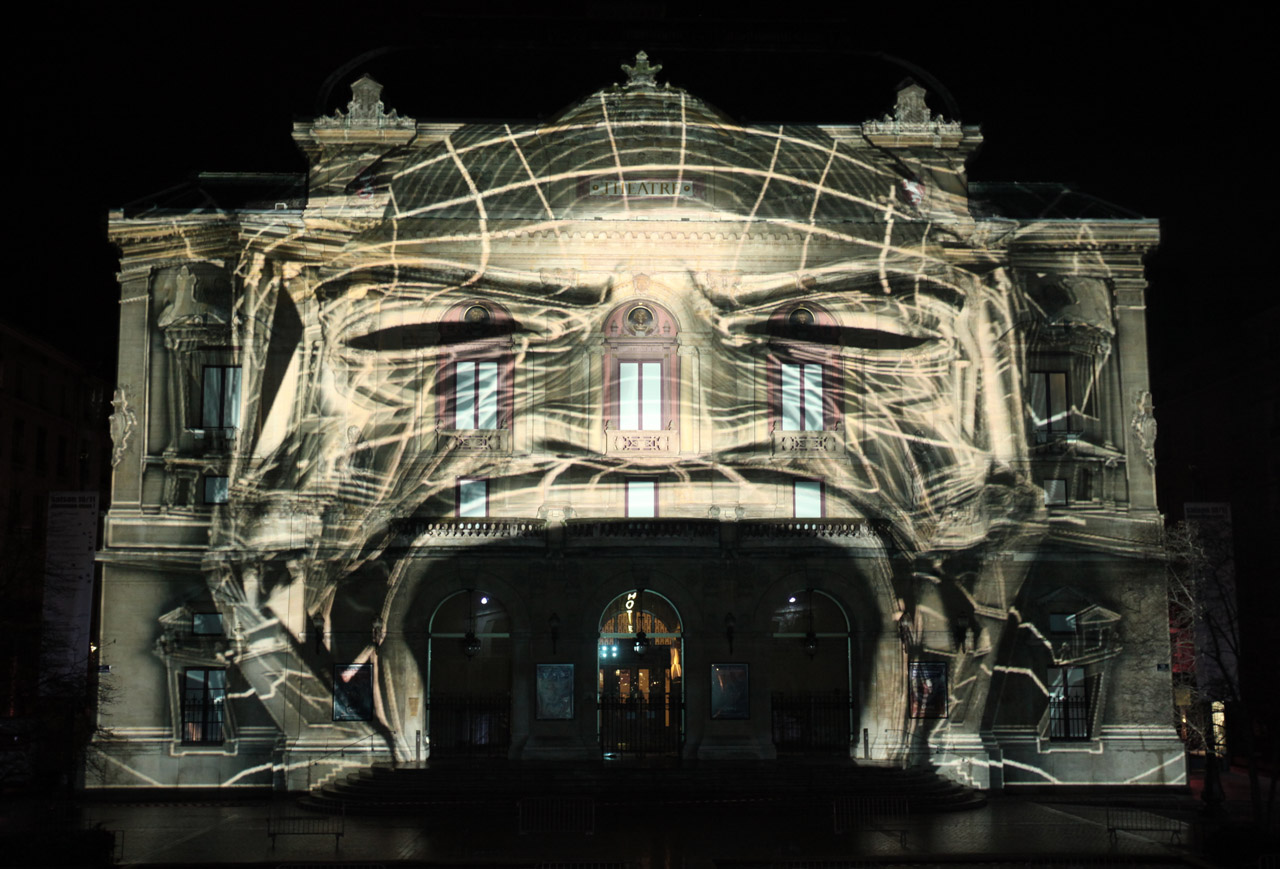
\includegraphics[width=0.75\textwidth]{./Cap2_videomapping/realcelestins_headshot.jpg}
		  \caption[http://mappingvideo.blogspot.com/]{Vista del efecto proyectado.}
		  \label{fig:Efecto2}
		\end{figure}
	\end{flushright}
\end{minipage}

Al utilizar videos para crear efectos es usual que se tenga en cuenta su posterior proyección, en particular la superficie donde se proyectará y el punto de vista desde donde se contemplará el espectáculo.
Un ejemplo en el que esta consideración es importante es cuando se pretende crear una ilusión tridimensional, pues la perspectiva de las formas proyectadas en el efecto debe ser coherente con la escena desde la óptica de los espectadores.

\begin{figure}[H]
  \centering
    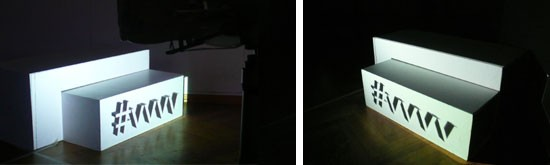
\includegraphics[width=0.7\textwidth]{./Cap2_videomapping/3dillusion}
  \caption[vvvv.org]{Izq. Ilusión tridimensional lograda. Der. No se logra la ilusión.}
  \label{fig:3dillusion}
\end{figure}

En este contexto se habla de mapeo, no como la salida a través de un equipo proyector, sino como la operación que logra una correspondencia entre una textura y una figura geométrica que no necesariamente coinciden en tamaño y forma. Para esto se definen coordenadas de textura en cada vértice de la figura geométrica que referencian distintas ubicaciones dentro de dicha textura.
Las coordenadas de las texturas tienen dos componentes: una horizontal y una vertical llamadas $UV$. Si el valor de estas componentes se normaliza entre $0$ y $1$ entonces la esquina superior izquierda de la textura se corresponderá con la coordenada $(0,0)$, la superior derecha con $(1,0)$, la inferior izquierda con $(0,1)$ y la inferior derecha con $(1,1)$.
Los vértices de una figura geométrica se asocian con coordenadas $UV$ que definen el punto de la textura que se corresponde sobre el vértice y mediante interpolación se logra mapear toda la textura a la figura geométrica.

Si bien es posible mapear una textura a cualquier figura geométrica, esta correspondencia es más directa utilizando un cuadrilátero ya que a cada uno de los vértices se lo hace corresponder con una esquina de la textura. A su vez el cuadrilátero es la figura básica en las aplicaciones\footnote{Las aplicaciones relevadas utilizan el cuadrilátero como figura básica. Ver apéndice: Aplicaciones relevadas.} de \emph{video mapping}.
Estos cuadriláteros se utilizan como piezas constructoras del espectáculo, cubriendo sectores del modelo sobre los cuales luego se aplican las texturas permitiendo crear los distintos efectos visuales.

\begin{figure}[H]
  \centering
    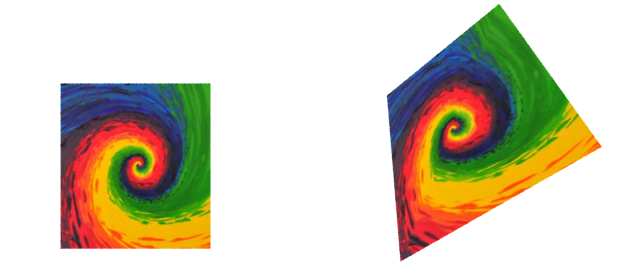
\includegraphics[width=0.7\textwidth]{./Cap2_videomapping/2dmapping}
  \caption[Imagen propia.]{Izq. Textura. Der. Cuadrilátero con textura mapeada.}
  \label{fig:2dmapping}
\end{figure}

\subsubsection{Proyección del espectáculo}
La principal dificultad encontrada en la etapa de la proyección del espectáculo es lograr que el modelo previamente generado se corresponda con la escena sobre la cuál se proyectará. El proceso que ajusta este modelo a proyectar con la superficie que representa es denominado calibración.
Los ajustes necesarios varían dependiendo del método utilizado para obtener el modelo. En caso de utilizar una fotografía, el proyector deberá ser ubicado de forma tal que el punto de vista de la cámara con la que se tomó coincida con el del proyector y así lograr la coincidencia del centro de proyección. Igualmente son necesarios ajustes ya que los lentes de la cámara y el proyector no necesariamente coinciden en el ángulo de visión.
Con el método de generación de figuras geométricas en el que se modelan las secciones de la superficie a mapear utilizando el mismo proyector, los ajustes se reducen a lograr la misma posición y orientación que tiene el proyector al momento de la captura de secciones, ya que las deformaciones relacionadas a los parámetros intrínsecos fueron implícitamente consideradas durante el proceso de captura.

En cualquiera de estos dos métodos, lograr que la posición y orientación del proyector coincidan con el punto de vista desde donde se obtuvo el modelo puede no ser una tarea sencilla. Esta tarea puede ser asistida, modificando la proyección mediante una homografía\footnote{Esto se extiende en la sección: Obtención de geometría} que es la transformación geométrica que permite corresponder puntos en dos planos de perspectiva distintos, logrando de esta manera ajustar el modelo proyectado a la superficie.
Este procedimiento deberá ser realizado nuevamente en caso de haber alteraciones en la posición y orientación del proyector ya que los parámetros de calibración obtenidos al lograr la correspondencia son particulares para una ubicación del proyector dada.

\subsection{Enfoque tridimensional}
\subsubsection{Modelo}
En el modelado tridimensional se representan cuerpos y superficies tridimensionales comúnmente representadas por medio de mallas de polígonos, utilizadas en disciplinas como visión computacional y computación gráfica. A diferencia de un modelo bidimensional, éste no depende de un punto de vista, lo que permite al diseñador visualizarlo desde diferentes ángulos mediante la definición de cámaras virtuales. Las entidades que conforman la malla son vértices, aristas, caras y atributos numéricos que representan la posición y normales de los vértices, coordenadas de textura y colores. Existen distintas topologías de mallas de polígonos siendo de las más utilizadas la que se basa en la cantidad de vértices que forman una cara.

\begin{minipage}{0.35\textwidth}
\begin{flushleft} \large
\begin{figure}[H]
  \centering
    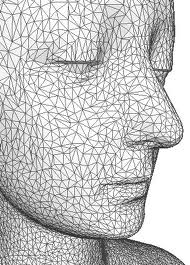
\includegraphics[width=0.7\textwidth]{./Cap2_videomapping/EjemploMallaTriangular}
  \caption[http://stochastix.wordpress.com/2008/07/15/bust-of-mystery]{Mallas triangulares.}
  \label{fig:mallas1}
\end{figure}
\end{flushleft}
\end{minipage}
\begin{minipage}{0.45\textwidth}
\begin{flushright} \large
\begin{figure}[H]
  \centering
    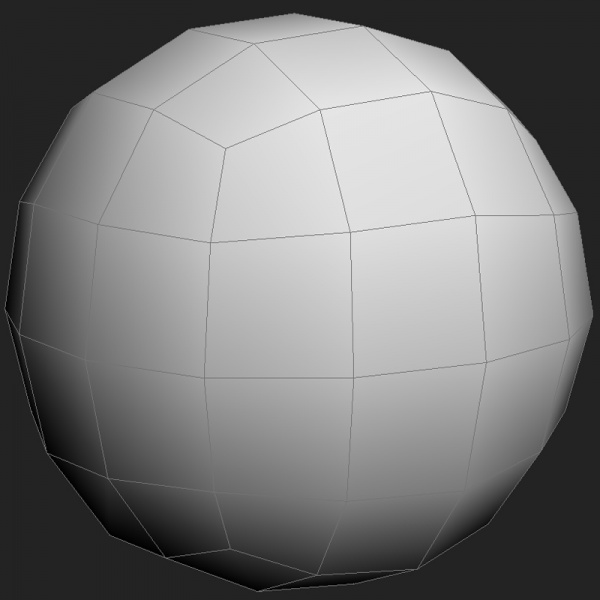
\includegraphics[width=0.75\textwidth]{./Cap2_videomapping/EjemploMalla4Vertices}
  \caption[http://www.fallingpixel.com]{Mallas de cuadriláteros.}
  \label{fig:mallas2}
\end{figure}

\end{flushright}
\end{minipage}

Técnicas como las de \emph{remeshing}, mediante la utilización de algoritmos específicos reducen la cantidad de vértices de la malla sin perder la representatividad de la superficie.
Un estudio de estas técnicas se presenta en el artículo \emph{Recent advances in compression of 3D meshes\cite{Mesh_building}}.
De esta forma se logra eficiencia en el manejo de las mallas que generalmente utilizan algoritmos cuyo orden varía dependiendo de la cantidad de vértices así como también se optimiza el almacenamiento de estas representaciones.

Los modelos tridimensionales se generan utilizando distintas técnicas cuya elección depende de varios factores como el nivel de detalle deseado, uso final del modelo y habilidades del usuario. Algunas de estas técnicas son:
\begin{itemize}
  \item Modelado utilizando polígonos: a partir de mallas que representan figuras primitivas, por ejemplo cubos o esferas, se podrán construir nuevas mallas aplicando transformaciones que modifican las aristas, vértices o caras.
  
  \item Modelado utilizando curvas: a partir de una jaula creada por curvas se aplican transformaciones para modificarla, manipulando sus puntos de control. Es utilizado en el modelado de automóviles, edificios y mobiliario, entre otros.

  \item Esculpido digital: técnica digital que simula el esculpido convencional mediante software especializado que provee una interfaz para modificar el modelo de forma detallada, oprimiendo y resaltando zonas de la superficie. Es utilizado para lograr efectos especiales en películas y video juegos logrando figuras y texturas complejas.

  \item Reconstrucción a partir de fotografías: se obtiene la representación de la superficie con una foto. Conociendo la escala de la imagen y mediante mediciones de los objetos fotografiados se extrapola y se obtiene la distancia entre dos puntos en la superficie. Es usada en arquitectura, ingeniería, geología, arqueología, etc.
  
  \item Reconstrucción utilizando hardware especializado: mediante escáneres tridimensionales se obtiene una nube de puntos que representa la superficie. El conjunto de puntos obtenido es denso, generalmente con redundancia y errores, es por esto que comúnmente se utilizan algoritmos específicos para reducir la nube de puntos \footnote{Esta técnica se ampliará en la sección Obtención de Geometía}.
\end{itemize}

Para las técnicas de modelado utlizando polígonos y curvas, algunas de las herramientas más populares son \emph{Maya}\cite{Maya}, \emph{3D Studio Max}\cite{3DStudioMax} y \emph{Blender}\cite{Blender}, mientras que para la realización de esculpido digital son también muy utilizadas \emph{3D-Coat}\cite{3DCoat}, \emph{ZBrush}\cite{Zbrush}, \emph{Sculptris}\cite{Sculptris} y \emph{Mudbox}\cite{Mudbox}. 

\begin{figure}[H]
  \centering
    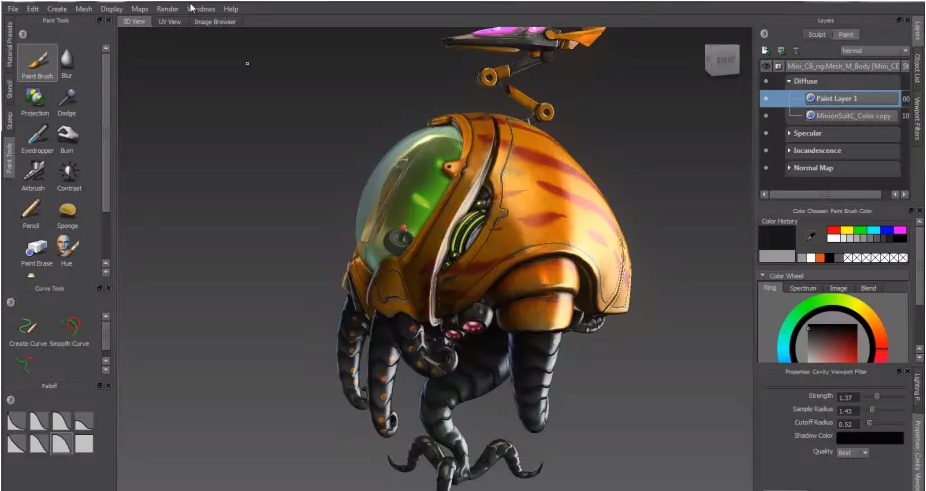
\includegraphics[width=0.7\textwidth]{./Cap2_videomapping/mudbox.png}
  \caption[http://usa.autodesk.com]{\emph{Mudbox}}
  \label{fig:Mudbox}
\end{figure}

\begin{figure}[H]
  \centering
    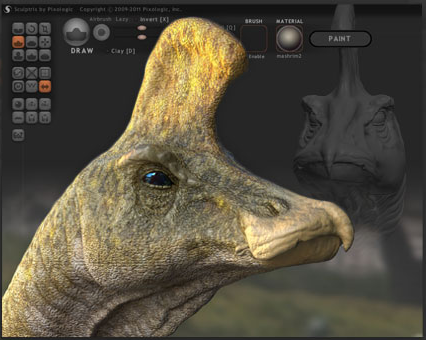
\includegraphics[width=0.7\textwidth]{./Cap2_videomapping/sculptris.png}
  \caption[http://www.pixologic.com/sculptris/]{\emph{Sculptris}}
  \label{fig:Sculptris}
\end{figure}
  
\subsubsection{Producción del espectáculo}
La producción del espectáculo en tres dimensiones agrega un nivel de abstracción adicional a la producción bidimensional. Esto permite que el diseñador cree un espectáculo transformando directamente los objetos del modelo tridimensional en contraposición al anterior enfoque en el que se transforman sus perspectivas.
Se plantea un cambio en la forma de trabajar en el espectáculo y planificar la producción, ya que el diseñador no estará restringido a considerar ubicación alguna de los proyectores.

El modo de trabajo se basa en mapear texturas sobre las caras de los objetos tridimensionales de forma análoga a como se realiza sobre figuras bidimensionales. En este tipo de modelos podría ser deseable mapear una textura de forma que abarque varias caras del mismo objeto tridimensional, por ejemplo, el conjunto de caras que representa la superficie lateral curva de un cilindro. Para lograrlo se deben mapear distintos sectores de la textura en cada una de las caras que conforman la superficie, utilizando coordenadas de textura en cada uno de los vértices.
La diferencia radica en que en el presente enfoque los vértices no se encuentran necesariamente en el mismo plano, por lo cual ajustar una textura bidimensional a este tipo de superficies no es directo.

Existen diversas técnicas que asisten en la tarea de definir las coordenadas de textura.
Una de ellas consiste en aproximar la superficie por una primitiva conocida, más simple, como ser un cubo, cilindro, esfera o plano. Para estas superficies existen funciones matemáticas que proyectan cada punto de la superficie a un plano, de esta forma se pueden determinar las coordenadas $UV$.
Un ejemplo de esto para esferas son las proyecciones utilizadas para representar el planisferio como la proyección cilíndrica equidistante presentada en el libro \emph{Flattening the Earth\cite{flatteningTheEarth}}.
Otra técnica es la denominada $UV$ \emph{unwrapping} que consiste en desenvolver una malla tridimensional, aplanándola sobre la textura. De esta manera el mapeo se realiza de forma más intuitiva ya que la superficie aplanada es bidimensional al igual que la textura. Esta técnica es soportada por la mayoría de los programas de edición de gráficos tridimensionales, los que proveen distintas herramientas para ajustar la forma en que se desenvuelve la textura.

\begin{figure}[H]
  \centering
    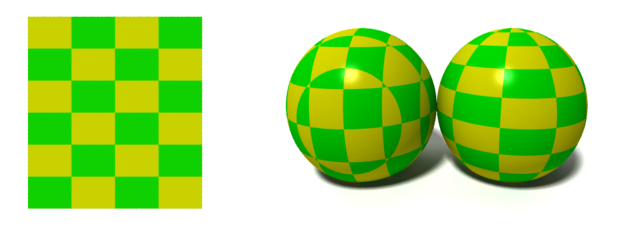
\includegraphics[width=0.7\textwidth]{./Cap2_videomapping/3dmapping}
  \caption[Imagen propia.]{Izq. Textura. Der. Esferas con distintos mapeos de la misma textura.}
  \label{fig:3dmapping}
\end{figure}

En la escena tridimensional los objetos son visualizados utilizando cámaras virtuales que fijan un punto de vista. En la salida gráfica se representará entonces la escena desde la perspectiva de una cámara virtual, permitiendo visualizarla desde distintos ángulos. Esto posibilita definir el punto de vista del proyector que reproducirá la salida gráfica en el momento que se desee. Un caso sería visualizar el resultado del espectáculo luego de producido y en este momento definir el punto de vista más conveniente.

Producir el espectáculo con este enfoque, es decir, transformando directamente los objetos y no sus perspectivas, permite escalar con mayor facilidad en la cantidad de proyectores a utilizar. Esto se logra agregando cámaras virtuales que definan más puntos de vista sin necesidad de modificar el modelo ni los efectos producidos.

Si bien se está abordando un enfoque tridimensional de la producción del espectáculo, existen casos en que es más sencilla la implementación de ciertos efectos tomando un enfoque en dos dimensiones, sobre todo cuando estos se aplican sobre regiones planas de la superficie. Es por esto que es muy común combinar ambos enfoques y utilizarlos de acuerdo a las necesidades del diseñador. Cabe aclarar que al combinar los enfoques se pierden las ventajas de definir el punto de vista del proyector luego de la etapa de producción por lo que los objetos bidimensionales y efectos sobre estos se deben definir una vez fijada la ubicación de los proyectores.

\subsubsection{Proyección del espectáculo}

En esta etapa se fija finalmente el punto de vista desde donde se proyectará, definiendo la ubicación y orientación de los proyectores.
Al igual que en el enfoque bidimensional, para lograr una correspondencia en la proyección de la escena con las superficies a proyectar se debe realizar una calibración que consiste en modificar los parámetros de ubicación, orientación y proyección de las cámaras virtuales.
La ubicación y orientación relativas de la cámara virtual y la escena deberán corresponderse a las del proyector con las superficies a proyectar.

%Agregar una seccion mas que redondee los 2 enfoques?%

\section{Obtención de geometría}

En esta sección se presenta la reconstrucción tridimensional automática de una superficie utilizando técnicas computacionales.
Se introducen distintos métodos que permiten la construcción automática de modelos, discutiendo sus características según propiedades de la superficie a representar y tecnologías utilizadas. Inicialmente se obtiene una nube de puntos correspondiente a la superficie, utilizando técnicas y dispositivos para este propósito, para luego procesar la información obtenida y construir una malla tridimensional. Mediante este procesamiento se obtienen propiedades adicionales como grupos de puntos que representan caras de una malla y las normales que identifican la orientación de la superficie.

\subsection{Obtención de la nube de puntos}

\subsubsection{Visión estéreo}

La visión estéreo se basa en el análisis de dos imágenes observadas desde puntos de vista ligeramente diferentes, de forma similar a la visión humana, para reconstruir la estructura tridimensional de una escena. Este método entra en la categoría de los métodos pasivos por no utilizar luz auxilar. El análisis de las imágenes se realiza por medio de algoritmos que han evolucionado en los últimos tiempos logrando la reconstrucción de escenas rápidamente. Es por esto que esta técnica es muy utilizada en implementaciones que necesitan respuesta en tiempo real.
Un primer paso es el preproceso de las imágenes donde se identifican sus principales características. Este análisis definirá que tipo de algoritmo se utilizará en el paso de correspondencia, ya que definirá las características que se estudiarán. Luego se resuelve el problema de correspondencia, en el que dadas dos imágenes de la escena, para todos los puntos de la primera se obtiene el punto correspondiente en la otra y se calcula la desigualdad de cada punto, es decir, la distancia en píxeles entre los puntos que se corresponden. Finalmente se calcula la profundidad del punto utilizando el método de triangulación\footnote{ver anexo de método de triangulación} en el cual se obtiene la distancia focal de cada punto a cada una de las cámaras\cite{StereoReview}.

Existen variedad de algoritmos que solucionan el problema de correspondecia y cálculo de desigualdad entre los puntos de las dos imágenes. Se pueden clasificar según el análisis de preproceso identificando características principales de las mismas destacándose dos estrategias\cite{StructureFromStereo}:
\begin{itemize}
   \item \emph{Separate area}: basada en correlación del brillo e intensidad. Se utilizan patrones de brillo aplicados a un píxel y sus vecinos utilizando principio de localidad. Las diferencias en la perspectiva de la imagen o cambios en luminosidad absoluta de la escena pueden generar errores.
   \item \emph{Features}: las características usadas para la correspondencia son aristas, puntos o segmentos dadas por cambios de intensidad de la imagen. Esta estrategia es más estable ante la variación de luminosidad absoluta y en la práctica la correspondencia es más rápida.
\end{itemize}

\begin{figure}[H]
  \centering
    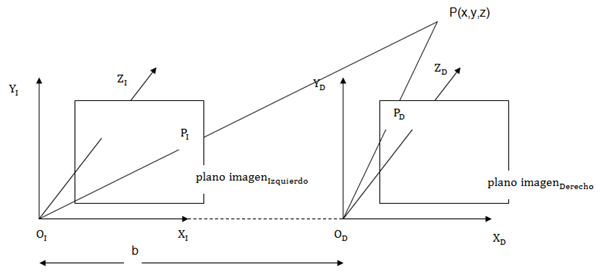
\includegraphics[width=0.5\textwidth]{./Cap2_videomapping/stereo.PNG}
  \caption[Structure from Stereo- A Review Umesh R. Dhond and J.K.Aggarwal 1989]{Geometría estéreo con ejes paralelos}
  \label{fig:Stereo}
\end{figure}
En la figura \ref{fig:Stereo} se muestra un caso particular de geometría estéreo que consta de ejes ópticos de las cámaras paralelos y en consecuencia los planos de imagen son coplanares. En los casos más comunes no se tienen estas características, y por ello es necesario introducir parámetros en los cálculos que hacen el ajuste del modelo \emph{pinhole\footnote{Ver apéndice modelo de cámara: modelo \emph{pinhole}}} al modelo de las cámaras reales.

\begin{figure}[H]
  \centering
    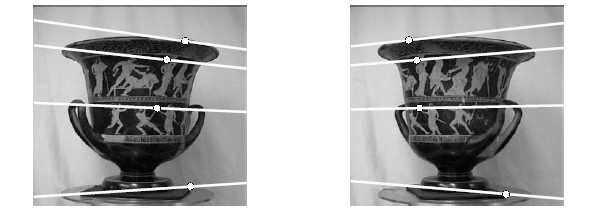
\includegraphics[width=0.5\textwidth]{./Cap2_videomapping/epipolar3.PNG}
  \caption[Geometría de Cámaras StereoReview pag 241. fig 9.3]{Dos imágenes con las líneas epipolares y puntos que se corresponden}
  \label{fig:Stereo2}
\end{figure}
En el caso mostrado en la figura \ref{fig:Stereo2} se ven los puntos correspondientes en cada imagen ubicados sobre las líneas epipolares\footnote{ver anexo de geometría epipolar}.

La principal desventaja del método de visión estéreo es que en caso de oclusión hay regiones que no tienen correspondencia en las dos imágenes, por esto no se puede resolver el problema de correspondencia para estas regiones.

\subsubsection{Luz estructurada}

Luz estructurada es una técnica de obtención de geometría tridimensional que consiste en la proyección de patrones sobre la superficie a capturar para luego analizar la deformación de los mismos y obtener una nube de puntos que la representan. Este método, a diferencia de visión estéreo, es un método activo ya que reemplaza la segunda cámara por un proyector de luz que proyecta patrones sobre la supericie a modelar.
Los patrones son capturados por la cámara de video para su posterior análisis, obteniendo información tridimensional de la posición, orientación y textura de la superficie\cite{SLightPatterns}.

Dependiendo de la superficie a escanear, los patrones proyectados pueden tener problemas de oclusión, baja reflexión y puntos reflejados fuera del alcance de la cámara. Como consecuencia, la pérdida de estos puntos proyectados impide resolver el problema de la correspondencia.
Estos problemas se pueden solucionar utilizando una codificación de patrones adecuada\cite{SLightCorrespondence}.

Según dependencia temporal los patrones se clasifican en:
\begin{itemize}
	\item Estáticos: El patrón es limitado para escenas estáticas en donde son necesarias proyecciones de varios patrones distintos. El movimiento de cualquier objeto de la escena mientras se realiza la obtención de los patrones proyectados producirá un error de correspondencia.
	\item Dinámicos: Los objetos en la escena se pueden mover por lo tanto es necesaria la utilización de un único patrón de proyección.
\end{itemize}

Clasificación según la luz proyectada:
\begin{itemize}
	\item Binaria: Cada uno de los puntos del patrón tiene dos posibles valores codificados con $0$ y $1$ respectivamente. Este valor representa opacidad y transparencia, ausencia o presencia de la luz proyectada en el objeto.
	\item Escala de grises: Cada punto del patrón tiene asociado un valor de gris que representa el nivel de trasparencia o nivel de opacidad del punto para la luz proyectada. En este caso son necesarios dos pasos. Primero se obtiene una imagen de la escena iluminada con la misma luz sin variar la intensidad y luego se obtiene la referencia de luz necesaria para cancelar el efecto de reflejo de la superficie que depende directamente del tipo de superficie. La necesidad de estos dos pasos contribuye a que este patrón también sea clasificado como estático.
	\item Color: Cada punto del patrón es asociado con un valor de tono. Los tonos deben ser bien diferenciados para alcanzar una segmentación eficiente. Este tipo de patrones son limitados por el color de la escena. En caso de presentar colores altamente saturados se producen pérdidas de regiones en el paso de segmentación que luego provocan errores en la decodificación.
\end{itemize}

Otra posible clasificación es según la discontinuidad en la profundidad de la superficie proyectada:
\begin{itemize}
	\item Periódica: La codificación se repite periódicamente a lo largo del patrón. Esta técnica se utiliza para reducir el número de bits que codifican el patrón. Como limitante la profundidad del objeto no puede ser mayor que la mitad de la longitud del período.
	\item Absoluta: Cada columna o fila del patrón proyectado tiene una única codificación. No sufre dependencia de discontinuidad de profundidad.
\end{itemize}

Un algoritmo que utiliza codificación binaria es el llamado \emph{Three Phase-Shifting} que utiliza tres ondas sinusoidales para la proyección del patrón. Este algoritmo fue presentado por Zhang\cite{ZhangS} e implementado por Kyle McDonalds en \cite{KyleMcDonald}. Dicho algoritmo es aplicable únicamente para superficies con curvas continuas, superficies disjuntas o con aristas pronunciadas serán capturadas de forma distorsionada.
\begin{figure}[H]
  \centering
    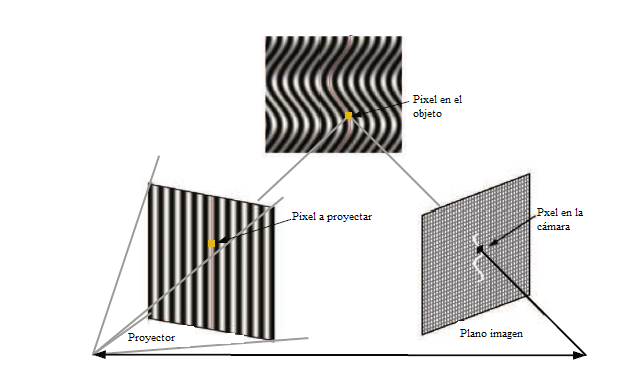
\includegraphics[width=0.8\textwidth]{./Cap2_videomapping/diagramaLS.png}
  \caption[Recent progresses on real-time 3D shape measurement using digital fringe projection techniques]{Instalación básica de proyección de patrones y sistema de \emph{Phase-Shifting}}
  \label{fig:phase21}
\end{figure}
\begin{figure}[H]
  \centering
    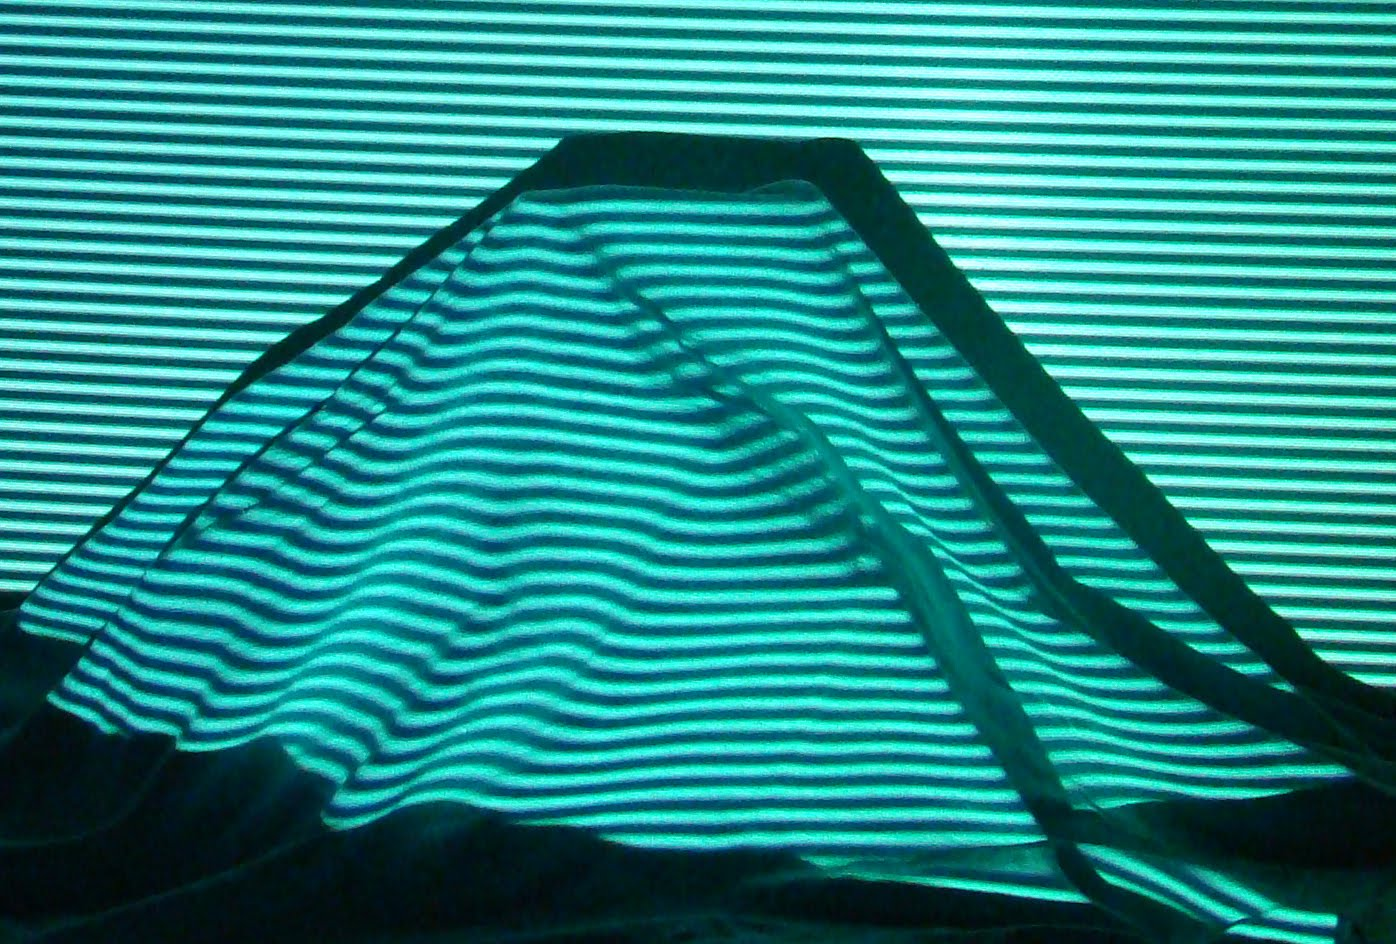
\includegraphics[width=0.8\textwidth]{./Cap2_videomapping/phase2.jpg}
  \caption[Imagen propia.]{Superficie con patrón proyectado}
  \label{fig:phase2}
\end{figure}

\paragraph{Calibración}

En esta sección se describe un método originalmente propuesto por Zhang\cite{ZhangS} para la calibración de una cámara y un proyector con el objetivo de capturar correctamente los patrones proyectados para su posterior análisis.
La calibración de la cámara requiere estimar inicialmente los parámetros del modelo de cámara \emph{pinhole}, por lo tanto se deben obtener los parámetros intrínsecos como distancia focal, punto principal y factores de escala, y los extrínsecos definidos por la matriz de rotación y vector de traslación de un punto en el espacio al sistema de coordenadas de la cámara.
Luego se debe capturar una secuencia de imágenes de un objeto simple, con un conjunto de características fijo y distinguible, y con un desplazamiento tridimensional conocido. Esto permite que cada imagen capturada durante el proceso de calibración provea de un conjunto de correspondencias de los puntos tridimensionales de la escena a puntos bidimensionales en el sistema de coordenadas de la cámara. Particularmente, en el método de Zhang, el objeto conocido que se observa es un tablero de damas plano en una o más orientaciones. De la secuencia capturada se pueden obtener los parámetros intrínsecos y luego, utilizando una sola toma de la secuencia, se obtienen los parámetros extrínsecos.
Para la calibracion del proyector, éste se modela como el inverso de una cámara, teniendo en cuenta que la luz viaja en la dirección opuesta y que un punto en el plano de la imagen se mapea a un rayo de luz saliente por el punto y por el centro de proyección.
Dado este modelo, la calibración se debe realizar de forma similar a la de una cámara, con la salvedad que en lugar de tomar imágenes de un tablero de damas fijo, se proyecta un tablero en una ubicación conocida y se toman imágenes del mismo utilizando la cámara para analizar las distorsiones. Este enfoque resulta ser una extensión directa del método de Zhang para calibración de cámaras.

Existen varias implementaciones de esta técnica de calibración basado en el modelo inverso de la cámara. Una de estas implementaciones es \emph{BYO3D}\cite{BYO3D}, que se encuentra disponible para \emph{MATLAB}\cite{MATLAB} y como una extensión a la biblioteca de visión computacional \emph{OpenCV}\cite{OpenCV}.

\subsubsection{Dispositivos de captura de geometría}

Un dispositivo para la captura de geometría en tres dimensiones cuenta con componentes de hardware y software que implementan las técnicas antes mencionadas.
En general, estos componentes son seleccionados de modo que optimicen las técnicas en las que se basan.
Un ejemplo de estos dispositivos es \emph{DAVID Structured Light Scanner\cite{DAVID}}, cuyo componente de software utiliza la técnica de luz estructurada y su hardware está compuesto por una cámara y un proyector de video. Otro es el caso \emph{Kinect} de \emph{Microsoft}, que también implementa la técnica de luz estructurada con la salvedad de que se reemplaza el proyector y la cámara de video por un emisor y una cámara de infrarrojos.

\begin{figure}[H]
  \centering
    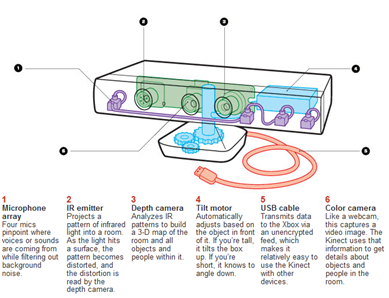
\includegraphics[width=0.7\textwidth]{./Cap2_videomapping/kinect.PNG}
  \caption[http://qph.cf.quoracdn.net/main-qimg-90d9a2ceb96f836e0b724027c2aba723]{Componentes de un sensor \emph{Kinect}}
  \label{fig:Kinect}
\end{figure}

En los últimos años se ha popularizado el uso de \emph{Kinect} por ser un dispositivo que se puede adicionar a la consola \emph{Xbox360} de \emph{Microsoft} con el objetivo de permitir que el usuario interactúe con la misma utilizando únicamente el movimiento de su cuerpo.
Para el análisis de las deformaciones de los rayos y construir el mapa de profundidad, mediante el emisor infrarrojo con el que viene equipado se proyectan patrones de luz por toda la escena y utilizando la cámara de profundidad se analizan las distorsiones. También se cuenta con una cámara convencional para analizar objetos o personas en la escena y para la detección de colores.

A mediados de 2011 fue presentada una interfaz de programación gratuita que permite utilizar \emph{Kinect} de forma directa en aplicaciones no licenciadas para diferentes propósitos, no limitándose a los videojuegos. Esto motiva la aparición de una variedad de aplicaciones que explotan las posibilidades del dispositivo \emph{Kinect}. Una de ellas es \emph{KinectFusion}\cite{KinectFusion}, biblioteca orientada a la reconstrucción tridimensional de objetos en tiempo real, con la posibilidad de que tanto éstos como el sensor estén en movimiento y con esto realizar capturas en 360 grados.

\subsection{Procesamiento de nube de puntos}

Al utilizar técnicas de obtención de geometría el resultado generado es una nube de puntos. Esta nube de puntos por lo general es densa, por lo que es necesario simplificar este modelo con el objetivo de eliminar redundancia y mejorar el rendimiento durante su procesamiento. Un problema adicional al volumen de la información obtenida es que comúnmente se introduce ruido, es decir, información distorsionada que no corresponde con puntos de la realidad. Para solucionar este problema se realiza un suavizado en el procesamiento de la nube de puntos\cite{PCloudSimplify}.

Las heurísticas existentes para reducir nubes de puntos pueden clasificarse en tres grandes grupos \cite{PntCloud}:
\begin{itemize}
   \item \emph{Clustering methods}: consiste en obtener grupos de la nube de puntos en donde cada grupo se remplaza por un conjunto de puntos representativos en él. Los grupos se pueden construir utilizando un enfoque incremental en el cual estos son creados iniciando por un punto aleatorio y agregando puntos vecinos hasta llegar a una cantidad establecida de elementos. Otra enfoque es el jerárquico, en donde se particiona el conjunto de puntos recursivamente hasta conseguir grupos de un tamaño predefinido.
   \item \emph{Iterative simplification}: se recorren iterativamente los puntos de la nube contrayendo parejas en un único punto. Se evalúa el error introducido, utilizando mínimos cuadrados, que se genera en la contracción comparándolo con el error que se obtendría al contraerse con otro punto vecino y eligiendo la contracción que introduce menor error al sistema. La simplificación se da por finalizada por haber logrado la cantidad de puntos deseada o por superar una cota$^\dagger$ de error a introducir en el sistema.
   \item \emph{Particle simulation}: se generan nuevos puntos que sustituyen la nube de puntos original. Se generan conjuntos de partículas que se mueven aleatoriamente en la superficie hasta lograr un balance.
\end{itemize}

Luego de simplificar la nube de puntos se construye un modelo tridimensional a partir de ella utilizando mallas de triángulos debido a la simplicidad de los algoritmos que dibujan este tipo de figuras geométricas. Esto permite que sean implementados fácilmente en hardware además del beneficio de que cualquier polígono con más de tres caras puede representarse como un conjunto de triángulos \cite{PCloudTriangle}.

A continuación se detallan los algoritmos asociados a cada paso de un típico procesamiento de malla que toma como entrada una nube de puntos, realiza un sub-muestreo y suavizado de la misma, calcula las normales en cada punto de la nube y finalmente aplica algoritmos de reconstrucción de la malla. Esto es implementado en bibliotecas como \emph{VcgLib}\cite{VCGLib} y \emph{CGAL}\cite{CGAL}.

\begin{figure}[H]
  \centering
    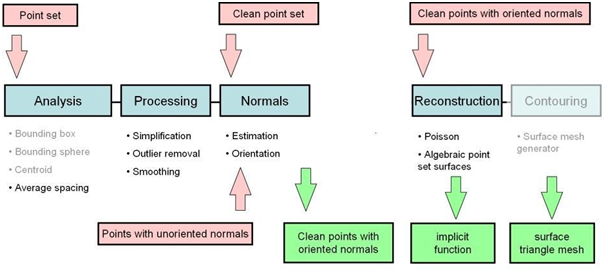
\includegraphics[width=0.5\textwidth]{./Cap2_videomapping/malla-flow.png}
  \caption{Flujo típico de procesamiento de nubes de puntos \cite{CGAL}}
  \label{fig:Mesh-CGAL}
\end{figure}

\subsubsection{Muestreo \emph{Poisson-disk}}

El muestreo de variables aleatorias es una técnica utilizada para una gran variedad de aplicaciones como procesamiento de imágenes y geometrías. Particularmente, el muestreo \emph{Poisson-disk} se utiliza para la ubicación aleatoria de objetos en mundos artificiales, algoritmos de texturas procedurales y procesamiento de geometrías o mallas. Esta técnica genera conjuntos de puntos con la propiedad de que sean suficientemente cercanos pero con la restricción de no estar más próximos unos de otros que una distancia mínima predeterminada.

\begin{figure}[H]
  \centering
    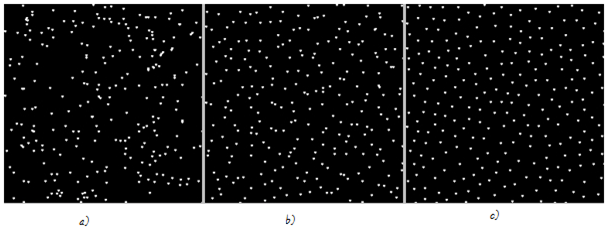
\includegraphics[width=0.5\textwidth]{./Cap2_videomapping/malla-poisson.png}
  \caption{a) Posición $x$ e $y$ generadas aleatoriamente. b) Imagen dividida en celdas. Puntos aleatorios generados en cada celda. c) Muestreo \emph{Poisson-disk} en dos dimensiones.}
  \label{fig:Mesh-Poisson}
\end{figure}

En líneas generales, este algoritmo genera puntos alrededor de los ya existentes en la muestra y valida si pueden ser agregados al conjunto final en caso de no violar la regla de la mínima distancia a los vecinos. Se genera una grilla en dos o tres dimensiones, dependiendo del escenario de aplicación, en la cuál cada celda contendrá al final del proceso a lo sumo un punto. Una grilla adicional es utilizada para realizar búsquedas rápidas y dos conjuntos de puntos son mantenidos durante el procesamiento para poder diferenciar los que han sido generados y los que aún necesitan procesamiento.
La implementación realizada en \emph{VcgLib} recibe tres parámetros:
\begin{itemize}
  \item 1) La cantidad de puntos en la muestra: El radio de cercanía es calculado en base a este parámetro.
  \item 2) El radio: Es utilizado para calcular el tamaño de la muestra óptimo en base a la malla inicial.
  \item 3) Sub muestreo: Indica si la muestra de Poisson es un subconjunto de la muestra inicial o si se deberán generar nuevos puntos aleatoriamente.
\end{itemize}

\subsubsection{Reconstrucción de normales}

Este algoritmo computa las normales en cada elemento de un conjunto de puntos sin la necesidad de explorar la conectividad de los triángulos. Por ello es muy útil para objetos tridimensionales sin información de caras.
Se detalla un pseudo-código del método:

\paragraph{Paso 1: }Identificar los planos tangentes para aproximar localmente la superficie y estimar así los vectores normales.


Para cada vértice:
  \begin{itemize}
    \item Calcular el centro geométrico del plano tangente en el punto como el promedio de los $K$ puntos más cercanos.
    \item Calcular la normal asociada al centro geométrico. Se utiliza la matriz de covarianza en el punto, contemplando los mismos $K$ vecinos más cercanos de la muestra y los valores y vectores propios de la matriz de covarianza. Finalmente, ordenando los vectores propios, la estimación del vector perpendicular corresponde al vector propio de menor valor. Este método es conocido como \emph{Principal Component Analysis (PCA)}.
  \end{itemize}

\paragraph{Paso 2: }Construir un grafo en donde cada punto está conectado a los $K$ vecinos más cercanos (grafo de Riemannian)


Se crea un grafo en cuyos nodos se guardan todas las aristas incidentes a los $K$ vecinos más cercanos. A cada arista se le asigna un peso igual al valor absoluto del producto escalar de la normal en el punto con la normal en cada uno de los $K$ vecinos:
   $$fabs(nodoActual->normal . K\_Vecinos[n]->normal)$$
\paragraph{Paso 3: }Calcular el árbol de expansión mínimo sobre el grafo de Riemannian y recorrerlo para orientar las normales.


Dado un grafo conexo, no dirigido, con sus aristas con un peso asignado, se llama árbol de expansión mínimo al sub-grafo con forma de árbol que conecta todos los nodos con un peso total mínimo conteniendo todos los nodos del grafo inicial. El grafo de entrada es el construido en el paso anterior y se utiliza el algoritmo de Kruskal$^\dagger$, uno de los varios algoritmos que resuelven el problema de encontrar un árbol de expansión mínima de un grafo.
Una vez construido el árbol de expansión, lo único que se hace es recorrerlo en orden e invertir el sentido de los vectores normales en caso de ser necesario. La condición para efectuar dicha corrección se basa en el ángulo del nodo siendo inspeccionado en comparación a todas las direcciones de las normales de los vecinos conectados a dicho nodo.

\subsubsection{Reconstrucción de malla de Poisson}

Para reconstruir la malla a partir de la nube de puntos y sus normales, se utiliza el algoritmo de reconstrucción de Poisson.
Se computa una función indicadora $\chi$ definida de la siguiente forma:

$$
\left\{ \begin{array}{rl}
 \chi = 1 & \mbox{ si puntos dentro del modelo} \\
 \chi = 0 & \mbox{ si puntos fuera del modelo}
       \end{array} \right.
$$

Luego, se obtiene una reconstrucción de la superficie mediante la extracción de la superficie de nivel en 3 dimensiones al nivel apropiado.
La estrategia se basa en la estrecha relación que hay entre los puntos de la muestra, orientados por sus normales, y la función indicadora de la muestra. Específicamente el gradiente de la función indicadora es un espacio de vectores, de valor nulo en todo el espacio excepto en puntos cercanos a la superficie, donde son iguales al vector normal a ella.
Es por eso que puntos orientados pueden ser vistos como muestras del gradiente de la función indicadora del modelo tridimensional en cuestión y es por este mismo motivo que el problema de reconstrucción de una malla puede ser visto como un problema de Poisson estándar, es decir, computar la función escalar $F$ cuya divergencia del gradiente se iguala a la divergencia del espacio de vectores de las normales.
